\chapter{Inheritance and Polymorphism}

%\fEnEmp{Inheritance} ဟာ ကလပ်စ်တစ်ခုကို အခြေခံပြီး အခြား ကလပ်စ်အသစ်တစ်ခု သတ်မှတ်လို့ရစေတဲ့ နည်းလမ်းတစ်ခု ဖြစ်တယ်။ \fEn{Inheritance} အသုံးပြုတဲ့အခါ နဂိုကလပ်စ်မှာ ပါဝင်တဲ့ \fEn{attribute} တွေနဲ့ မက်သဒ်တွေကို နောက်တစ်ခါ ပြန်ရေးဖို့မလိုဘဲ ကလပ်စ်အသစ်က ဆက်ခံရရှိနိုင်မဲ့အပြင် လိုအပ်သလို ထပ်မံ တိုးချဲ့ ဖြည့်စွက်တာ \fEn{(extension)} နဲ့ နဂိုရှိရင်းကို ပြင်ဆင်တာ \fEn{(modification)} လည်း  လုပ်ဆောင်လို့ရမှာဖြစ်တယ်။


\fEnEmp{Inheritance} ဟာ ရှိထားပြီး ကလပ်စ်တစ်ခုရဲ့ \fEn{attribute} နဲ့ မက်သဒ်တွေကို အခြားကလပ်စ်ကနေ ဆက်ခံယူဖို့ ဖြစ်နိုင်စေတယ်။ ကလပ်စ်တစ်ခုမှာ ရေးထားတဲ့ ပရိုဂရမ် ကုဒ်တွေကို ထပ်ခါထပ်ခါ ရေးစရာမလိုဘဲ ပြန်လည် အသုံးပြုလို့ရစေတဲ့ နည်းလို့လည်း ယူဆနိုင်တယ်။ ဆက်ခံရရှိတဲ့  \fEn{attribute} နဲ့ မက်သဒ်တွေအပြင် အသစ် ထပ်ထည့်တာ၊ နဂိုရှိရင်းကို ပြင်ဆင်တာလည်း ကလပ်စ်အသစ်က  လုပ်ဆောင်လို့ရမှာဖြစ်တယ်။ \fEn{Object-oriented programming} မှာ \fEn{inheritance} ဟာ အရေးအပါဆုံး သဘောတရားတစ်ခု ဆိုရင်လည်း မမှားဘူး။ ဂိမ်းရေးတဲ့ လိုက်ဘရီတွေ၊ \fEn{Graphical User Interface (GUI)} အတွက် လိုက်ဘရီတွေ အသုံးပြုမယ်ဆိုရင် \fEn{inheritance} သဘောတရားက မသိမဖြစ်ပါပဲ။  ဒီအခန်းအတွက် \fEn{inheritance} အသုံးချ ဥပမာအနေနဲ့ \fEn{‘Breakout’} လို့ခေါ်တဲ့ ဂိမ်းလေးတစ်ခုကို \fEn{Arcade} လိုက်ဘရီနဲ့ ရေးထားတာကို နောက်ပိုင်းမှာ လေ့လာကြရမှာပါ။

ရှေ့အခန်းမှာ ဖော်ပြခဲ့တဲ့ \fEn{has-a} အပြင် \fEn{object-oriented programming} မှာ အရေးပါတဲ့ နောက် \fEn{relationship} တစ်မျိုးက \fEnEmp{is-a} ဖြစ်ပါတယ်။ \fEn{Is-a relationship} ရှိတဲ့ အရာတွေကို \fEn{inheritance} နဲ့ ထင်ဟပ်ဖော်ပြနိုင်တယ်။  ဘတ်စ်ကားသည် ကားဖြစ်သည်။ ကားသည် ယာဉ်ဖြစ်သည်။ ယာဉ်၊ ကားနဲ့ ဘတ်စ်ကားတို့အကြား ဆက်စပ်မှုဟာ \fEn{is-a relationship} ဖြစ်တယ်။  \fCode{Vehicle}\fEn{,} \fCode{Car} နဲ့ \fCode{Bus} ကလပ်စ်တွေဟာ အစဉ်အလိုက် \fEn{inherit} လုပ်ယူနိုင်တာကို တွေ့ရမှာပါ။


%ပေါ်လွင်တဲ့ ဥပမာတစ်ခု ပြရမယ်ဆိုရင် ဘတ်စ်ကားနဲ့ ကားအကြား ဆက်နွယ်မှုဟာ \fEn{is-a} \fEn{relationship} ပါ။ “ဘတ်စ်\allowbreak ကားသည် ကားဖြစ်သည်”။ ဒါကြောင့် ဘတ်စ်ကားမှာ ကားရဲ့ လက္ခဏာရပ်တွေ အားလုံးရှိရမှာပါ။ ထိုနည်းတူစွာ လော်ရီကားသည်လည်း  ကားဖြစ်တဲ့အတွက် သူ့မှာလည်း ကားရဲ့ လက္ခဏာရပ်တွေ ရှိရမှာ ဖြစ်တယ်။ ဘီးတွေပါမယ်၊ မောင်းလို့ရတယ်၊ ဘရိတ်အုပ်လို့ ရမယ် စသည်ဖြင့်ပေါ့။ ဒီလို ယေဘုယျ ကားဖြစ်ခြင်း ဂုဏ်အင်္ဂါရပ်တွေအပြင် ဘတ်စ်ကားသီးသန့် ကားဂုဏ်အင်္ဂါရပ်တွေ၊ လော်ရီကားသီးသန့် ကားဂုဏ်အင်္ဂါရပ်တွေလည်း ပါရှိရမယ်။ ဒါမှလည်း ဘတ်စ်ကား (သို့) လော်ရီကားလို့ ခေါ်လို့ရမယ်။ ဥပမာ ဘတ်စ်ကားဆိုရင် ခရီးသည်အတွက် ထိုင်ခုံတွေ များများပါမယ်။  ခရီးသည် အများဆုံး ဘယ်လောက်ဆံ့လဲ သတ်မှတ်ချက်ရှိတယ်။ အတက်အဆင်းအတွက် တံခါးတွေရှိမယ်။ လော်ရီကားဆိုရင်တော့ ကုန်အတွက်သီးသန့်ပဲ။ ကုန်တန်ချိန် အများဆုံးဘယ်လောက် တင်လို့ရလဲ စတာတွေရှိမယ်။ 

 


\section{Inheritance ဥပမာ ‘\fSecCodeBf{Account} Class Hierarchy’}
ဘဏ်အကောင့် အမျိုးအစား အမျိုးမျိုး ရှိပါတယ်။ အတိုးနှုန်း၊ တစ်နေ့တာ လုပ်ဆောင်နိုင်တဲ့ \fEn{transaction} အကြိမ်အရေအတွက်၊ အနည်းဆုံး ထားရှိရမဲ့ ငွေပမာဏ၊ လက်ရှိ လက်ကျန်ငွေထက် ပိုထုတ်လို့ ရ/မရ \fEn{(overdraft)} စတဲ့အချက်တွေ အကောင့်တစ်မျိုးနဲ့တစ်မျိုး မတူကြပါဘူး။ 

ဥပမာ \fEn{savings account} (ငွေစုအကောင့်) ဆိုရင် ဘဏ်တိုးရမယ်။ တစ်နေ့တာ \fEn{transaction} အကြိမ်အရေအတွက်ရော ထုတ်ယူနိုင်တဲ့ ငွေပမာဏပါ အကန့်အသတ်ရှိတယ်။ ဒါကြောင့် ဒီအကောင့် အမျိုးအစားက လုပ်ငန်းသုံးအတွက် အဆင်မပြေဘူး။   \fEn{Current account} ကတော့ စီးပွားရေး လုပ်ငန်းတွေအတွက် အဓိက ရည်ရွယ်တယ်။ \fEn{Transaction} အကန့်အသတ်မရှိဘူး။ လိုသလောက် ထုတ်ယူလို့ရတယ်။ \fEn{Overdraft} လို့ခေါ်တဲ့ ကိုယ့်မှာရှိတာထက် (အကန့်အသတ်တော့ရှိတာပေါ့) ပိုထုတ်လို့ရတယ်။ \fEn{Current account} ကို ဘဏ်က အတိုးပေးလေ့မရှိဘူး။ 

\fCode{SavingAccount} နဲ့ \fCode{CurrentAccount} ကလပ်စ်ကို အောက်ပါအတိုင်း သတ်မှတ်နိုင်ပါတယ်။ ကလပ်စ်နှစ်ခုကို နှိုင်းယှဉ်ကြည့်ရင် တူညီတဲ့အပိုင်းတွေ ပါဝင်နေတာ တွေ့ရမှာပါ။  နှစ်ခုလုံးမှာ \fCode{deposit} မက်သဒ်က တူတူပါပဲ။  \fCode{\_holder}\fEn{,} \fCode{\_balance}\fEn{,} \fCode{\_acc\_number}  ဗေရီရေဘဲလ်တွေ ပါဝင်တာချင်းလည်း တူတယ်။ ကွာခြားချက်တချို့ကိုလည်း တွေ့ရပါတယ်။ \fCode{withdraw} မက်သဒ် နှစ်ခု မတူကြဘူး။  \fCode{\_txn\_cnt\_\allowbreak tot}\fEn{,} \fCode{\_txn\_amt\_tot} နဲ့ \fCode{provide\_interest} တို့ကို \fCode{SavingAccount} မှာပဲ တွေ့ရတယ်။ တစ်ဖက်မှာလည်း \fCode{\_overdraft\_amt} နဲ့ \fCode{is\_overdrafted} တို့ကိုတော့ \fCode{CurrentAccount} မှာ တွေ့မှာဖြစ်ပြီး \fCode{SavingAccount} မှာ မပါပြန်ဘူး။
%
\begin{py}
class SavingAccount:
    def __init__(self, holder, acc_number, balance):
        self._holder = holder
        self._acc_number = acc_number
        self._balance = balance
        self._txn_cnt_tot = 0
        self._txn_amt_tot = Decimal(0.00)

    def deposit(self, amt):
        if amt <= Decimal(0.00):
            raise ValueError('Invalid amount for deposit!')
        self._balance += amt

    def withdraw(self, amt):
        if self._txn_amt_tot >= Decimal(500_000.00):
            raise ValueError('Daily withdraw limit exceeds!')
        if self._txn_cnt_tot >= 5:
            raise ValueError('Daily transaction count exceeds!')
        if amt > self._balance:
            raise ValueError('Not enough balance!')
        self._balance -= amt

    def provide_interest(self):
        """complex logic for interest calculation"""
        pass
\end{py}
%
\betweenminted{\medskipamount}
%
\begin{py}
class CurrentAccount:
    def __init__(self, holder, acc_number, balance):
        self._holder = holder
        self._acc_number = acc_number
        self._balance = balance
        self._overdraft_amt = Decimal(1_000_000.00)

    def deposit(self, amt):
        if amt <= Decimal(0.00):
            raise ValueError('Invalid amount for deposit!')
        self._balance += amt

    def withdraw(self, amt):
        if amt > (self._balance + self._overdraft_amt):
            raise ValueError('Not enough balance!')
        self._balance -= amt

    def is_overdrafted(self):
        return self._overdraft_amt < Decimal(0.00)
\end{py}
%
 
ဒီကလပ်စ်နှစ်ခုမှာ ထပ်နေတဲ့ တူညီတဲ့ကုဒ်တွေကို  တစ်ခါပဲ ရေးဖို့လိုမယ်ဆိုရင် ပိုပြီးအဆင်ပြေမှာပါ။ ဒီလိုအခြေအနေမျိုးမှာ \fEn{inheritance} က ဘယ်လို အထောက်အကူပြုလဲ ကြည့်ရအောင်။ ထပ်နေတဲ့ တူညီတဲ့ကုဒ်တွေကို ဘုံထုတ်လိုက်ပြီး ကလပ်စ်တစ်ခု သတ်မှတ်ပါမယ်။ 
%
\begin{py}
from decimal import Decimal

class Account:
    def __init__(self, holder, acc_number, balance):
        self._holder = holder
        self._acc_number = acc_number
        self._balance = balance

    def deposit(self, amt):
        if amt <= Decimal(0.00):
            raise ValueError('Invalid amount for deposit!')
        self._balance += amt
\end{py}
%
\fCode{CurrentAccount} နဲ့ \fCode{SavingAccount} က  တူညီတဲ့ အပိုင်းတွေ \fCode{Account} ကလပ်စ်မှာ ခွဲထုတ်ထားတာ သတိပြုကြည့်ပါ။  ဒီအပိုင်းတွေကို \fEn{inherit} လုပ်ယူပါမယ်။
%
\begin{py}
class CurrentAccount(Account):
    def __init__(self, holder, acc_number, balance, overdraft_amt):
        super().__init__(holder, acc_number, balance)
        self._overdraft_amt = overdraft_amt

    def withdraw(self, amt):
        if amt > (self._balance + self._overdraft_amt):
            raise ValueError('Not enough balance!')
        self._balance -= amt

    def is_overdrafted(self):
        return self._balance < Decimal(0.00)
\end{py}
%

\fCode{CurrentAccount} က \fCode{Account} ကို  \fEn{inherit} လုပ်မှာဖြစ်တာကြောင့် ကလပ်စ်သတ်မှတ်တဲ့အခါ အခုလို ရေးရပါမယ်
%
\begin{py}
class CurrentAccount(Account):
\end{py}
%
\fCode{Account} ကို \fEnEmp{superclass} လို့ခေါ်ပြီး သူ့ဆီကနေ ဆက်ခံယူမဲ့ \fCode{CurrentAccount} ကို  \fEnEmp{subclass} လို့ခေါ်ပါတယ်။ ပေးမဲ့ကလပ်စ်က \fEn{superclass} ၊ ယူမဲ့ ကလပ်စ်က \fEn{subclass} ပေါ့။ \fEnEmp{parent} နဲ့ \fEnEmp{child} လို့လည်းခေါ်တယ်။

\fEn{Subclass} \fEn{initialize} လုပ်တဲ့အခါ \fEn{superclass} အပိုင်းကိုလည်း  \fEn{initialize} လုပ်ဖို့လိုတယ်။ ဒီအတွက် \fEn{superclass} \mintinline{text}|__init__| ကို အခုလို ခေါ်ရပါတယ်
%
\begin{py}
# call __init__ method of the superclass
super().__init__(holder, acc_number, balance)
\end{py}
%
\fCode{\_holder}\fEn{,} \fCode{\_acc\_number}\fEn{,} \fCode{\_balance} \fEn{instance variable} တွေက ဆက်ခံရရှိထားတာပါ။ ၎င်းတို့ကို \fEn{initialize} လုပ်ဖို့အတွက်  \fEn{superclass}  \fEn{initializer} ကို ခေါ်ရပါမယ်။ \fEn{Subclass} က တိုက်ရိုက် မလုပ်ရပါဘူး။  \fEn{Subclass} ကိုယ်ပိုင် \fEn{instance variable} တွေကိုတော့ ပုံမှန်အတိုင်း \fEn{initialize} လုပ်နိုင်တယ်။
%
\begin{py}
self._overdraft_amt = overdraft_amt
\end{py}
%
 

\fCode{deposit} မက်သဒ်ကို \fEn{superclass} ကနေ \fCode{CurrentAccount} က ဆက်ခံရရှိမယ်။  \fCode{withdraw} နဲ့ \fCode{is\_overdrafted} က ကိုယ်ပိုင်ရှိမယ်။ ဒီမက်သဒ်နှစ်ခုမှာ \fCode{self.\_balance} ကို သုံးထားတာ တွေ့ရမှာပါ။  ဆက်ခံရရှိတဲ့ \fEn{instance variable} တွေကို \fEn{subclass} မက်သဒ်ထဲမှာ \fCode{self} နဲ့ ရည်ညွှန်းအသုံးပြုလို့ ရတယ်။  

\fCode{SavingAccount} ကိုအောက်ပါအတိုင်း သတ်မှတ်ပါတယ်။ တစ်နေ့တာ \fEn{transaction} အကြိမ်အရေအတွက်နဲ့ ထုတ်ယူတဲ့ ပမာဏအတွက်  \fCode{\_txn\_cnt\_tot} နဲ့ \fCode{\_txn\allowbreak \_amt\_tot} \fEn{instance variable} တွေ ထပ်ဖြည့်ထားတယ်။ (\fCode{\_txn\_cnt\_tot} နဲ့ \fCode{\_txn\allowbreak \_amt\_tot} ကို တစ်နေ့တာကုန်ဆုံးတိုင်း သုညဖြစ်အောင် ပြန်လုပ်ထားဖို့ လိုပါလိမ့်မယ်။ အခုဥပမာမှာ ဒီကိစ္စအတွက် ထည့်မစဉ်းစားထားပါဘူး)။
%
\begin{py}
class SavingAccount(Account):
    def __init__(self, holder, acc_number, balance):
        super().__init__(holder, acc_number, balance)
        self._txn_cnt_tot = 0
        self._txn_amt_tot = Decimal(0.00)

    def withdraw(self, amt):
        if self._txn_amt_tot >= Decimal(200_000.00):
            raise ValueError('Daily withdraw limit exceeds!')
        if self._txn_cnt_tot >= 30:
            raise ValueError('Daily transaction count exceeds!')
        if amt > self._balance:
            raise ValueError('Not enough balance!')
        self._balance -= amt
        self._txn_cnt_tot += 1
        self._txn_amt_tot += amt

    def provide_interest(self):
        """complex logic for interest calculation"""
        pass
\end{py}
%


\fEn{Saving} နဲ့ \fEn{current} အပြင် သတ်မှတ်ကာလအတွင်း မထုတ်ဘဲထားရတဲ့ \fEn{fixed deposit} ၊ အသေးစား လုပ်ငန်းတွေအတွက် \fEn{SME} စတဲ့ အခြားအကောင့် အမျိုးအစားတွေလည်း ရှိတယ်။ ဒီအကောင့်တွေနဲ့ သက်ဆိုင်တဲ့ ကလပ်စ်တွေကလည်း  \fCode{Account} ကို \fEn{inherit} လုပ်နိုင်ပါတယ်။ 


\section{Overriding}
\fEn{Superclass} ကနေ ဆက်ခံရရှိထားတဲ့ မက်သဒ်ကို \fEn{subclass} မှာ ပြင်ဆင်သတ်မှတ်တာကို  \fEnEmp{method overriding} လို့ ခေါ်ပါတယ်။ \fEn{Deposit} လုပ်တဲ့အခါ \fEn{current account} က အနည်းဆုံး ဆယ်သိန်းဖြစ်မှ လက်ခံတယ်ဆိုပါစို့။ ဆက်ခံ ရထားတဲ့ မူလ \fCode{deposit} မက်သဒ်က ဒီလိုအပ်ချက်နဲ့ မကိုက်ညီတော့ဘူး။  အခုလို အခြေအနေမျိုးမှာ ဆက်ခံယူမဲ့ \fCode{CurrentAccount} ဟာ  \fCode{deposit} မက်သဒ်ကို လက်ရှိလိုအပ်ချက်နဲ့ ကိုက်ညီအောင် \fEn{override} လုပ်နိုင်ပါတယ်။ 

%
\begin{py}
class CurrentAccount(Account):
    def __init__(self, holder, acc_number, balance):
        super().__init__(holder, acc_number, balance)
        super._holder = holder
        self._overdraft_amt = Decimal(1_000_000.00)
       
    # override deposit method
    def deposit(self, amt):
        if amt <= Decimal(1_000_000.00):
            raise ValueError('Deposit at least 1,000,000 to current acc!')
        self._balance += amt

    # other methods
\end{py}
%
မက်သဒ်တစ်ခုကို ဆက်ခံရရှိတဲ့အတိုင်း အသုံးပြုလို့ အဆင်မပြေတဲ့အခါ \fEn{subclass}  က   \fEn{override} လုပ်နိုင်ပါတယ်။ \fEn{Subclass} အများစုက ဆက်ခံရရှိတဲ့အတိုင်း အသုံးပြုလို့ရပြီး တချို့ အနည်းစုကပဲ   \fEn{override} ရတဲ့အခါ ကုဒ်တွေထပ်နေတာ သိသိသာသာ လျော့သွားမှာပါ။

ဆက်ခံရရှိတဲ့အတိုင်း အသုံးပြုလို့ရနိုင်ပေမဲ့ \fEn{optimization} အတွက် \fEn{override} လုပ်ရတာလည်း  ရှိတယ်။   \fEn{Polygon} ပါတ်လည်နားရှာတဲ့ နည်းလမ်းကို \fEn{rectangle} အတွက်လည်း သုံးလို့ရပေမဲ့ \fEn{rectangle} အတွက် သီးသန့်ဖော်မြူလာ $2 \times (width + height)$ က ပိုရှင်းလင်းပြီး တွက်ချက်ရပိုမြန်မှာ အမှန်ပါပဲ။ ဒါကြောင့် စွမ်းဆောင်ရည်အတွက်  \fCode{Rectangle} ကလပ်စ်မှာ \fCode{perimeter} ကို \fEn{override} လုပ်ဖို့ ဆုံးဖြတ်နိုင်ပါတယ်။

%
\begin{py}
import math

class Polygon:
    def __init__(self, vertices):
        self.vertices = vertices

    def perimeter(self):
        perimeter = 0
        num_vertices = len(self.vertices)
        for i in range(num_vertices):
            x1, y1 = self.vertices[i]
            x2, y2 = self.vertices[(i + 1) % num_vertices]
            perimeter += math.sqrt((x2 - x1) ** 2 + (y2 - y1) ** 2)
        return perimeter

class Rectangle(Polygon):
    def __init__(self, width, height):
        # Define vertices for a rectangle assuming bottom-left corner at (0, 0)
        vertices = [(0, 0), (width, 0), (width, height), (0, height)]
        super().__init__(vertices)
        self.width = width
        self.height = height

    def perimeter(self):
        # Overriding the perimeter method for performance
        return 2 * (self.width + self.height)
\end{py}
%

\fEn{Inheritance} နဲ့ \fEn{method overriding} ကို ပရိုဂရမ်တစ်ခုရဲ့ စထရက်ချာကို ထိန်းကွပ်ပေးဖို့ အသုံးပြုတာကိုလည်း တချို့လိုက်ဘရီတွေမှာ တွေ့ရတယ်။ ဥပမာ \fEn{Arcade} လိုက်ဘရီနဲ့ ဂိမ်းရေးတဲ့အခါ သူ့မှာပါတဲ့ ကလပ်စ်တွေကို \fEn{inherit} လုပ်ပြီး ကိုယ်လိုချင်တဲ့ ပုံစံနဲ့ အလုပ်လုပ်အောင် မက်သဒ်တွေကို လိုအပ်သလို \fEn{override} လုပ်ပေးရတယ်။  ဒီအခန်း နောက်ပိုင်းမှာ \fEn{Arcade} လိုက်ဘရီနဲ့ ဂိမ်းလေးတစ်ခု တည်ဆောက်တဲ့အခါ  တွေ့ရမှာပါ။

\section{Multilevel Inheritance}
ကလပ်စ် $A$ ကို $B$ က ဆက်ခံထားမယ်။ တစ်ခါ $B$ ကို $C$ က ထပ်ဆင့် ဆက်ခံယူမယ်။ ဒီလို အဆင့်ဆင့် \fEn{inherit} လုပ်တာကို \fEnEmp{multilevel inheritance} လို့ခေါ်တယ်။ ကလပ်စ် $C$ ဟာ $B$ နဲ့ $A$ နှစ်ခုလုံးရဲ့ \fEn{attribute} နဲ့ မက်သဒ်တွေကို ရရှိမှာပါ ($A$ မှာ ရှိတာတွေကို $B$ ကနေတစ်ဆင့် ရတာ)။ ရှေ့က ဥပမာမှာ \fEn{inheritance} \fEn{level}  နှစ်ခုတွေ့ရတယ်။ အပေါ်အဆင့်မှာ \fCode{Account}\fEn{,} အောက်တစ်ဆင့်မှာ သူ့ကိုဆက်ခံယူထားတဲ့ \fCode{SavingAccount} နဲ့ \fCode{CurrentAccount} ရှိတယ်။  \fCode{SavingAccount} နဲ့ \fCode{CurrentAccount} ကို ဆက်ခံထားတဲ့ ကလပ်စ်တွေ နောက်တစ်ဆင့်ရှိလာရင် သုံးဆင့်ဖြစ်သွားမှာပါ။ 


%
\begin{py}
class SavingAccount(Account):
    def __init__(self, holder, acc_number, balance):
        super().__init__(holder, acc_number, balance)
        self._txn_cnt_tot = 0
        self._txn_amt_tot = Decimal(0.00)

    def provide_interest(self):
        """complex logic for interest calculation"""
        pass
\end{py}
%
\betweenminted{\medskipamount}
%
\begin{py}
class SuperSavingAccount(SavingAccount):
    def __init__(self, holder, acc_number, balance):
        super().__init__(holder, acc_number, balance)

    def withdraw(self, amt):
        if self._txn_amt_tot >= Decimal(200_000.00):
            raise ValueError('Daily withdraw limit exceeds!')
        if self._txn_cnt_tot >= 30:
            raise ValueError('Daily transaction count exceeds!')
        if amt > self._balance:
            raise ValueError('Not enough balance!')
        self._balance -= amt
        self._txn_cnt_tot += 1
        self._txn_amt_tot += amt
\end{py}
%
\betweenminted{\medskipamount}
%
\begin{py}
class FamilySavingAccount(SavingAccount):
    def __init__(self, holder, acc_number, balance):
        super().__init__(holder, acc_number, balance)

    def withdraw(self, amt):
        if self._txn_amt_tot >= Decimal(600_000.00):
            raise ValueError('Daily withdraw limit exceeds!')
        if self._txn_cnt_tot >= 30:
            raise ValueError('Daily transaction count exceeds!')
        if amt > self._balance:
            raise ValueError('Not enough balance!')
        self._balance -= amt
        self._txn_cnt_tot += 1
        self._txn_amt_tot += amt
\end{py}
%

\section{Class Hierarchy and UML}

\section{Is-A Relationship and Inheritance}


\section{အသုံးချ ဥပမာ (၁) Breakout Game}
ဒီအခန်းအတွက် အသုံးချဥပမာက \fEn{Breakout} လို့ခေါ်တဲ့ ရိုးရှင်းတဲ့ ဂိမ်းလေးတစ်ခု တည်ဆောက်ပါမယ်။ \fEn{Breakout} ဂိမ်းဟာ ကမ္ဘာကျော် \fEn{Apple} ကုမ္ပဏီ ပူးတွဲတည်ထောင်သူ \fEn{Steve Wozniak} ဒီဇိုင်းလုပ်ခဲ့တဲ့ ဂန္ထဝင်ဂိမ်းတစ်ခု ဖြစ်ပါတယ်။ ဗားရှင်းတွေအမျိုးမျိုး ရှိပေမဲ့ အဓိကအနှစ်သာရကတော့ ရွေ့နေတဲ့  ဘောလုံးကို \fEn{paddle} ပြားနဲ့ လိုက်ဖမ်းပြီး အစီအရီရှိနေတဲ့ အုတ်ခဲတွေ အားလုံးကို ကုန်တဲ့အထိ ဖျက်ရတာပါ။  ဂိမ်းစစချင်း အနေအထားကို ပုံ  (\fRefNo{\ref{fig:breakout}}) မှာ တွေ့ရပါမယ်။ အပေါ်ပိုင်းမှာက အုတ်နံရံပေါ့။ ဘောလုံးက အောက်ကိုကျလာမယ်။ \fEn{paddle} ပြားနဲ့ လိုက်ဖမ်းရမယ်။ ဘောလုံးက \fEn{paddle}\fEn{,} အုတ်ခဲ၊ ဘယ်/ညာ/အပေါ် ဘောင်တွေနဲ့ ဝင်တိုက်ရင် ပြန်ကန်ထွက်တယ်။ အုတ်ခဲတွေက ဘောလုံးနဲ့ တိုက်မိရင် ပျက်သွားမယ်။ ဘောလုံးကို မဖမ်းလိုက်နိုင်လို့ \fEn{paddle} ပြားအောက်ဘက် ကျသွားရင် ရှုံးမယ် (အောက်ဘက်ကျသွားရင် ပြန်ကန်မထွက်ဘူး)။ အုတ်ခဲတွေ ကုန်တဲ့ထိ ဘောလုံးမကျသွားအောင် ထိန်းထားနိုင်ရင် အနိုင်ရမှာဖြစ်တယ်။ 

%
\begin{figure}[tbh!]
\begin{tikzpicture}
  \node[anchor=south west,inner sep=0] (image) at (0,0)
  {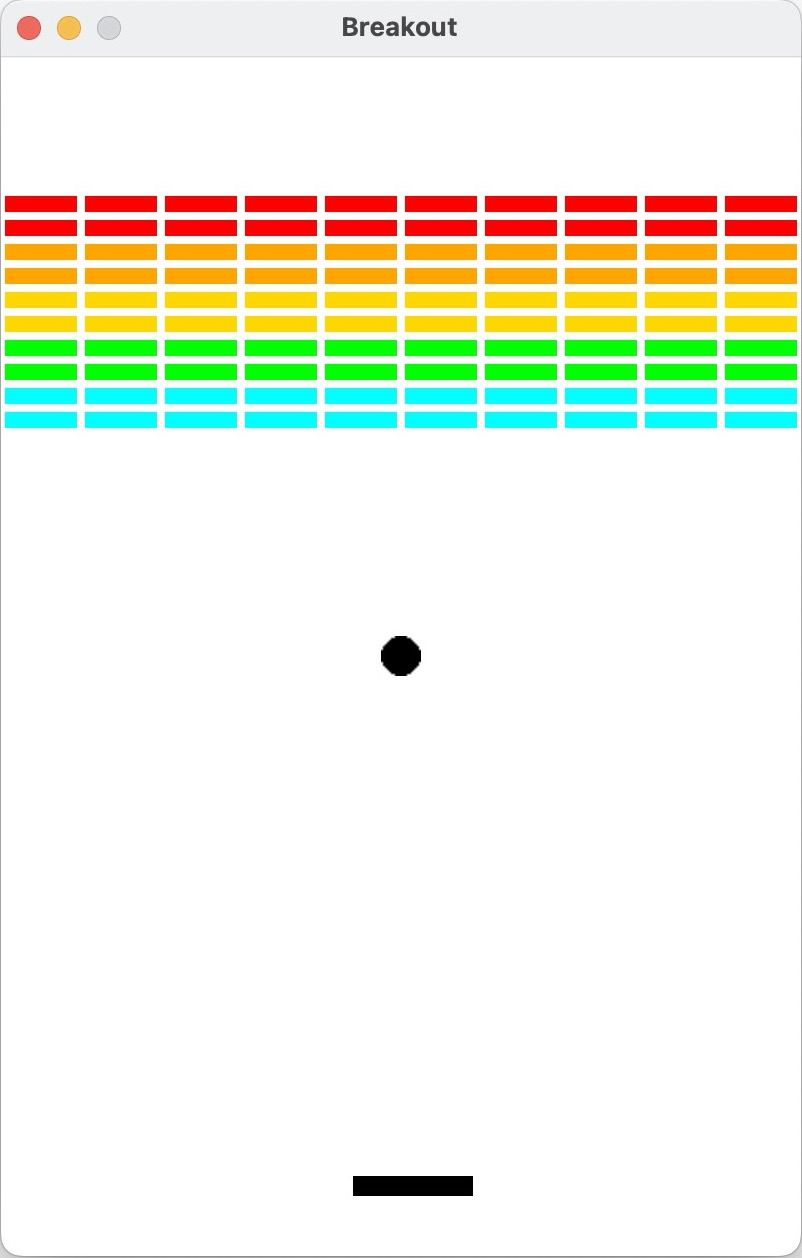
\includegraphics[width=.5\textwidth, clip]{images/ch10/breakout.jpg}};
  \drawshadow{image}
\end{tikzpicture}
\caption{} 
\label{fig:breakout}
\end{figure}
%

\fEn{Arcade} လိုက်ဘရီနဲ့ ရေးမှာပါ။ \fEn{Arcade} လိုက်ဘရီဟာ \fEn{inheritance} ကို အခြေခံထားတယ်။ \fCode{Window}\fEn{,} \fCode{View}\fEn{,} \fCode{Sprite} စတဲ့ ကလပ်စ်တွေကို လိုက်ဘရီကပေးထားတယ်။ ဂိမ်းတစ်ခုရေးတဲ့အခါ ဒီကလပ်စ်တွေကို \fEn{inherit} လုပ်ပြီး လိုအပ်တဲ့ မက်သဒ်တွေကို \fEn{override} လုပ်ပေးရုံပဲ။ လိုက်ဘရီက ပရိုဂရမ်ကို အကြမ်းထည် စထရက်ချာ ချထားပေးတယ်။ အဲ့ဒီ စထရက်ချာထဲမှာ ကိုယ်တိုင်စိတ်ကြိုက် ဖန်တီးချင်တဲ့နေရာတွေကို ပြင်ဆင်ဖြည့်စွက်လို့ရအောင် လုပ်ပေးထားတာလို့ ယူဆနိုင်တယ်။ ကြိုတင်သိထားဖို့ လိုအပ်တာတွေ တစ်ဆင့်ချင်း အရင်ကြည့်ရအောင်။

\subsection*{\fSubSecCodeBf{arcade.Window}}
\fCode{Window} ကလပ်စ်ဟာ ဂရပ်ဖစ် \fEn{window} တစ်ခုကို ကိုယ်စားပြုတယ်။ ဂရပ်ဖစ်ရုပ်ပုံတွေ ဆွဲဖို့နဲ့ အန်နီမေးရှင်း လုပ်ဖို့ လိုအပ်တာတွေ ဒီကလပ်စ်မှာ ထောက်ပံပေးထားတယ်။ ဒါ့အပြင် မောက်စ်၊ ကီးဘုဒ် စတဲ့ \fEn{input device} တွေနဲ့ ဂိမ်းကို ကွန်ထရိုးလ်လုပ်လို့ရစေမဲ့ နည်းလမ်းတွေလည်း ပါတယ်။

\fEn{Arcade} ပရိုဂရမ်တစ်ခုကို \fEn{run} တဲ့အခါ \fCode{Window} မှာ ပါတဲ့  \fCode{on\_draw} မက်သဒ်ကို တစ်စက္ကန့် အကြိမ် ခြောက်ဆယ် ခေါ်ပေးတယ်။ သူ့နဂိုအတိုင်း \fCode{on\_draw} မက်သဒ်က ဘာမှ လုပ်ဆောင်မပေးဘူး။ ကိုယ့်လိုချင်တဲ့ ဂရပ်ဖစ်ပုံ ဖော်ဖို့ \fCode{Window} ကို \fEn{inherit} လုပ်ပြီး \fEn{override} လုပ်ပေးရမယ်။  အပြာရောင် ဘောလုံးတစ်ခု အလယ်ဗဟိုမှာ ဆွဲမယ်ဆိုပါစို့ $\ldots$

%
\begin{py}
# File: arcade_blue_circle.py
import arcade
from arcade.color import *

WIN_WIDTH = 640
WIN_HEIGHT = 480

class MyGame(arcade.Window):

    def __init__(self, width, height, title):
        super().__init__(width, height, title)
        arcade.set_background_color(arcade.color.ALMOND)

    def on_draw(self):
        self.clear()
        arcade.draw_circle_filled(WIN_WIDTH / 2, WIN_HEIGHT / 2, 20, BLUE)

window = MyGame(WIN_WIDTH, WIN_HEIGHT, "Show Blue Circle")
arcade.run()
\end{py}
%
\fCode{on\_draw} ကို အခုလို  \fEn{override} လုပ်နိုင်ပါတယ်။ ဒီပရိုဂရမ် \fEn{run} တဲ့အခါ \fCode{on\_draw} ကို တစ်စက္ကန့်တိုင်း တစ်စက္ကန့်တိုင်းမှာ အကြိမ်ခြောက်ဆယ် \fEn{(60 frames per second)} တောက်လျှောက် ခေါ်နေမှာပါ။ ပရိုဂရမ် \fEn{window} မပိတ်မချင်းပေါ့။ ဒီလိုဖြစ်အောင် \fEn{Arcade} လိုက်ဘရီက လုပ်ပေးထားတာ။ ဒီအတွက် သီးခြားရေးဖို့ မလိုဘူး။ \fCode{Window} ကလပ်စ်ကို \fEn{inherit} လုပ်ပြီး \fCode{on\_draw} ကို \fEn{override} လုပ်ပေးရင် ရပြီ။ \fCode{clear} မက်သဒ်ကိုလည်း \fEn{superclass} \fCode{Window} ကနေ ဆက်ခံရထားတာ။ \fEn{Window} ပေါ်မှာ ရှိတဲ့ ဂရပ်ဖစ်အားလုံးကို ရှင်းပေးပြီး သတ်မှတ်ထားတဲ့ နောက်ခံရောင် ဖြည့်ပေးတဲ့ မက်သဒ်ပါ။  အန်နီမေးရှင်းအတွက် ဒီမက်သဒ်က အရေးကြီးတယ်ဆိုတာ တွေ့ရပါမယ်။ 

မောက်စ် (သို့) ကီးဘုဒ်နဲ့ ဘောလုံးကို ရွှေ့လို့ရအောင်လည်း လုပ်လို့ရတယ်။ ခက်ခဲတဲ့ ကိစ္စတွေကို \fCode{Window} က အဆင်သင့် လုပ်ထားပေးတာပါ။ ဒါဟာ အထူးအဆန်း ဖြစ်နေနိုင်ပါတယ်။ ဘယ်လိုများလုပ်ထားလဲ အကြမ်းဖျဉ်း သဘောတရား နားလည်ချင်တယ်ဆိုရင် အောက်ပါ ဥပမာကို လေ့လာကြည့်ပါ 
%
\begin{py}
class ConsolePrinter:
    def __init__(self, times):
        self._times = times
        
    def do_before(self):
        print("Checking if everything is ready.")
        
    def do_after(self):
        print("Doing cleaning up.")

    def do_my_task(self):
        self.do_before()
        for i in range(self._times):
            self.my_task()
        self.do_after()

    # do nothing    
    def my_task(self):
        pass


class MyConsolePrinter(ConsolePrinter):
    def __init__(self, times, text):
        super().__init__(times)
        self._text = text

    # to print as you want
    def my_task(self):
        print(self._text)


printer = MyConsolePrinter(15, 'Hello')
printer.do_my_task()
\end{py}
%
\fCode{ConsolePrinter}  မှာ \fCode{my\_task} ကလွဲလို့ ကျန်မက်သဒ်တွေအားလုံး အပြည့်အစုံရေးထားတာ တွေ့ရမှာပါ။ \fCode{do\_my\_task} က \fCode{my\_task} ကိုခေါ်ထားတယ်။ \fCode{MyConsolePrinter} က ထုတ်ပေးချင်တဲ့ စာသားအတွက် \fCode{my\_task} ကို \fEn{override} လုပ်ထားတာကို ဂရုပြုပါ။ ဒီသဘောတရားအတိုင်း \fEn{Arcade} လိုက်ဘရီက \fCode{Window}\fEn{,} \fCode{View}\fEn{,} \fCode{Sprite} စတဲ့ ကလပ်စ်တွေကလည်း ဒီသဘောတရားပဲ။ ဂိမ်းတစ်ခုအတွက် လိုအပ်ချက်တွေကို ပြင်ဆင်ပေးထားတယ်။ ပုံစံချပေးထားတယ်။ အသုံးပြုသူက ဒီကလပ်စ်တွေကို \fEn{inherit} လုပ်ပြီး သူ့ဂိမ်း လိုအပ်ချက်အတိုင်း ဖြစ်အောင် မက်သဒ်တွေကို \fEn{override} လုပ်ပြီး စိတ်ကြိုက်ဖန်တီးယူရတာ။


\subsection*{အန်နီမေးရှင်း}
စောစောက ပရိုဂရမ်မှာ စက်ဝိုင်းကို ညာဘက်ဘက်အပေါ်ကို ရွေ့သွားအောင် အန်နီမေးရှင်း လုပ်မယ်ဆိုပါစို့။ \fCode{on\_draw} လုပ်တဲ့ အခါတိုင်းမှာ လက်ရှိ $x$ နဲ့ $y$ တန်ဖိုးကို နည်းနည်းချင်း တိုးပေးနိုင်ပါတယ်။ နမူနာအနေနဲ့ $x$ ကို \fEn{2 pixels} နဲ့ $y$ ကို \fEn{1 pixel} တိုးပေးပါမယ်။
%
\begin{py}
# File: arcade_moving_circle.py
import arcade
from arcade.color import *

WIN_WIDTH = 640
WIN_HEIGHT = 480
RADIUS = 15


class MyGame(arcade.Window):

    def __init__(self, width, height, title):
        super().__init__(width, height, title)
        self._circle_x = WIN_WIDTH / 2
        self._circle_y = WIN_HEIGHT / 2
        arcade.set_background_color(arcade.color.ALMOND)

    def on_draw(self):
        self.clear()
        self._circle_x += 2     # move 2 pixels to the right
        self._circle_y += 1     # move 1 pixels upwards
        arcade.draw_circle_filled(self._circle_x,
                                  self._circle_y,
                                  RADIUS,
                                  BLUE)


window = MyGame(WIN_WIDTH, WIN_HEIGHT, "Moving Circle")
arcade.run()
\end{py}
%


\subsection*{\fSubSecCodeBf{Sprite}}
ဂိမ်းတစ်ခုမှာ ပါဝင်တဲ့ ဇာတ်ကောင်တွေ၊ အရာဝတ္ထုပစ္စည်းတွေကို \fCode{Sprite} ကလပ်စ်ကို  \fEn{inherit} လုပ်ပြီး ကိုယ်စားပြုနိုင်ပါတယ်။ တစ်ခုနဲ့တစ်ခု ဝင်တိုက်တာ \fEn{(collision)} ၊  အပေါ်/အောက် (သို့) ဘယ်/ညာလှည့်တာ၊  အရာဝတ္ထုတွေကို အုပ်စုလိုက် ရွေ့လျားစေတာ စတာတွေကို အလွယ်တကူ လုပ်ဆောင်လို့ရအောင် \fCode{Sprite} ကလပ်စ်က ထောက်ပံ့ပေးထားတယ်။ \fEn{Window} ဘောင် တစ်ဖက်ဖက်နဲ့ ဝင်တိုက်ရင် ဘောလုံးက ပြန်ကန်ထွက်တဲ့ အန်နီမေးရှင်းဥပမာကို ကြည့်ရအောင် $\ldots$
%
\begin{py}
# File: arcade_bouncing_ball.py
import arcade
SCREEN_WIDTH = 680
SCREEN_HEIGHT = 480


class Ball(arcade.Sprite):

    def update(self):
        # rotate the sprite
        self.angle += 1
        # move the sprite
        self.center_x += self.change_x
        self.center_y += self.change_y

        if self.left < 0:
            self.change_x *= -1

        if self.right > SCREEN_WIDTH:
            self.change_x *= -1

        if self.bottom < 0:
            self.change_y *= -1

        if self.top > SCREEN_HEIGHT:
            self.change_y *= -1
\end{py}
%

\fCode{center\_x}\fEn{,} \fCode{center\_y} က \fCode{Sprite} ဗဟိုမှတ် တည်နေရာ။ \fCode{change\_x}\fEn{,} \fCode{change\_y} က အန်နီမေးရှင်းလုပ်ရင် နည်းနည်းချင်း ရွှေ့ပေးရမဲ့ $x$ နဲ့  $y$ ပမာဏ။ \fCode{Sprite} အမြန်နှုန်းနဲ့ ဦးတည်ရာကို ဒီနှစ်ခုရဲ့ တန်ဖိုးနဲ့ ထိန်းညှိပေးနိုင်တယ်။ \fCode{left}\fEn{,} \fCode{right}\fEn{,} \fCode{top}\fEn{,} \fCode{bottom} \fEn{attribute} တွေကတော့   \fCode{Sprite} ရဲ့ ဘယ်/ညာ $x$ တန်ဖိုးနဲ့  အထက်/အောက် $y$ တန်ဖိုးတွေကို ဖော်ပြတယ်။ ဒီ ဗေရီရေဘဲလ်တွေ အားလုံးကို \fEn{superclass} \fCode{Sprite} ကနေ ဆက်ခံရရှိထားတာ။ 

ဘယ် (သို့) ညာဘက် ဘောင်နဲ့ ထိရင် \fCode{change\_x} ကို အပေါင်းအနှုတ် ပြောင်းပြန် လုပ်ပေးရပါမယ်။ အထက် (သို့) အောက် ဘောင်နဲ့ ထိရင် \fCode{change\_y} ကို ပြောင်းပြန် လုပ်ပေးရပါမယ်။ ပုံ (\fRefNo{\ref{fig:ch10bouncing}}) မှာ ကြည့်ပါ။

\fCode{Ball} ကလပ်စ်မှာ \mintinline{text}|__init__| မက်သဒ် မပါဘူး။ (\fEn{Subclass} မှာ \mintinline{text}|__init__| မပါရင် အော့ဂျက်ဖန်တီးတဲ့အခါ ဆက်ခံရရှိထားတဲ့ \fEn{superclass} \mintinline{text}|__init__| ကိုပဲခေါ်ပါတယ်)။ 

\begin{figure}[tbh!]
\begin{tikzpicture}
\draw [very thick] (0,0)--(10,0)--(10,6)--(0,6)--cycle;

\node at (3.5,4) [below] {$(+,+)$};
\node at (6.5,4) [below] {$(+,-)$};
\draw[-{Latex[length=3mm]}] (3.5,4)--(5,6);
\draw[-{Latex[length=3mm]}] (5,6)--(6.5,4);

\node at (4.5,2) [above] {$(-,-)$};
\node at (1.5,2) [above] {$(-,+)$};
\draw[-{Latex[length=3mm]}] (4.5,2)--(3,0);
\draw[-{Latex[length=3mm]}] (3,0)--(1.5,2);

\node at (8,4.5) [left] {$(+,-)$};
\node at (8,1.5) [left] {$(-,-)$};
\draw[-{Latex[length=3mm]}] (8,4.5)--(10,3);
\draw[-{Latex[length=3mm]}] (10,3)--(8,1.5);
\end{tikzpicture}
\caption{ဘောင်နဲ့တိုက်တဲ့အခါ velocity လက္ခဏာ ပြောင်းလဲပုံ} 
\label{fig:ch10bouncing}
\end{figure}



\fCode{MyGame} ကလပ်စ်မှာ ဒီ ဘောလုံးကို ဘယ်လို အသုံးပြုထားလဲ ဆက်စပ်ကြည့်ပါ။ 
\begin{py}
# File: arcade_bouncing_ball.py
class MyGame(arcade.Window):

    def __init__(self, width, height, title):
        super().__init__(width, height, title)

        self._ball = Ball('ball.png', 0.2)

        self._ball.center_x = SCREEN_WIDTH / 2
        self._ball.center_y = SCREEN_HEIGHT / 2
        self._ball.change_x = 2
        self._ball.change_y = 1
        arcade.set_background_color(arcade.color.AIR_FORCE_BLUE)

    def on_draw(self):
        self.clear()
        self._ball.draw()

    def on_update(self, delta_time):
        self._ball.update()


window = MyGame(SCREEN_WIDTH, SCREEN_HEIGHT, "Bouncing Ball")
arcade.run()
\end{py}
%

\fCode{Sprite} အော့ဘ်ဂျက် ဖန်တီးတဲ့အခါ \fEn{image file} နံမည်နဲ့ \fEn{scale factor} ထည့်ပေးရပါတယ်။ ဘောလုံးကို \fEnSnd{ball.png} ဖိုင်၊ \fEn{scale factor} $0.2$ နဲ့ 
%
\begin{py}
self._ball = Ball('ball.png', 0.2)
\end{py}
%
ဖန်တီးတယ်။  \fEn{Image file} က ကုဒ်ဖိုင်နဲ့ ဖိုဒါတစ်ခုထဲမှာ ရှိရပါမယ်။ ဒါက အလွယ်နည်းကို ပြောတာပါ။ အခြားဖိုဒါမှာ ထားလို့ရပေမဲ့ နည်းနည်း ပိုရှုပ်လို့။

\fCode{Sprite} ရွေ့လျားတာနဲ့ \fEn{collision} ဖြစ်တဲ့ ကိစ္စတွေအတွက် အဓိက ဂိမ်းလော့ဂျစ်ကို  \fCode{on\_update} မက်သဒ်မှာ ရေးပေးရမယ်။ ဒါလည်းပဲ တကယ်က ဆက်ခံထားတဲ့ \fCode{on\_update} ကို  \fEn{override} လုပ်တာပါ။  ဒီမက်သဒ်ကိုလည်း တစ်စက္ကန့် အကြီမ်ခြောက်ဆယ် အလိုအလျောက် ခေါ်ပေးပါတယ်။ ဒါပေမဲ့ \fCode{on\_draw}  ရည်ရွယ်ချက်ချင်း မတူပါဘူး။ \fCode{on\_draw} က စခရင်ကိုပဲ \fEn{refresh} လုပ်ပေးတာ။ တစ်နည်းအားဖြင့် \fEn{window} ပေါ်မှာ ဂရပ်ဖစ်ပုံပဲ ဖော်ပေးတာ။ ဂိမ်းလော့ဂျစ်နဲ့ သက်ဆိုင်တာတွေ မလုပ်ဘူး။ \fCode{on\_update} ကျတော့ ပုံဆွဲတဲ့ကိစ္စကို မလုပ်ဘူး။ ဂိမ်းလော့ဂျစ်သီးသန့် လုပ်ဆောင်တယ်။ ဒီမက်သဒ်နှစ်ခု လုပ်ဆောင်ပေးတဲ့ တာဝန်ကို ခွဲခြားထားရပါမယ်။ ဂိမ်းမှာပါဝင်တဲ့ \fCode{Sprite} အားလုံးရဲ့ \fEn{state} ကို \fEn{update} လုပ်ပေးခြင်းဟာ \fCode{on\_update} ရဲ့ အဓိကတာဝန်တွေထဲက တစ်ခုအပါအဝင် ဖြစ်တယ်။ အခုဥပမာမှာ ဘောလုံးရဲ့ \fEn{state} ကို
%
\begin{py}
self._ball.update()
\end{py}
%
ခေါ်ပြီး \fEn{update} လုပ်ပေးထားတယ်။

\fCode{on\_update} မက်သဒ် \fCode{delta\_time} ပါရာမီတာကို ရှင်းပြဖို့ ကျန်ပါသေးတယ်။ \fCode{on\_update} ကို ခေါ်တဲ့အခါ နောက်ဆုံးခါ်ခဲ့တဲ့ အချိန်နဲ့ အခုခေါ်တဲ့ အချိန်ကြား ကွဟချက်ကို \fCode{delta\_time} အနေနဲ့ ထည့်ပေးတယ်။ \fEn{Arcade} လိုက်ဘရီ နောက်ကွယ်က အလုပ်လုပ်ပုံ သဘောတရားအရ ထည့်ထားတဲ့ ပါရာမီတာဖြစ်ပြီး လိုက်ဘရီ သုံးတဲ့သူအနေနဲ့ အသေးစိတ်သိဖို့ မလိုအပ်ပါဘူး။ \fCode{on\_update} ကို \fEn{override} လုပ်တဲ့အခါ \fCode{delta\_time} ပါရာမီတာ မကျန်ခဲ့ရင် ရပါပြီ။


\subsection*{Event Handling}
မောက်စ်၊ ကီးဘုဒ်၊ \fEn{joystick} စတဲ့ \fEn{input device} တွေနဲ့ ဂိမ်းကို ထိန်းချုပ်ဖို့အတွက်လည်း \fCode{Window} ကလပ်စ်က လွယ်အောင်လုပ်ထားတယ်။ \fCode{on\_mouse\_motion}\fEn{,} \fCode{on\_mouse\_press}\fEn{,} \fCode{on\_key\_press} စတဲ့ မက်သဒ်တွေကို \fEn{override} လုပ်ရုံပါပဲ။ အဖြစ်အပျက် တစ်စုံတစ်ခု \fEn{(event)} ကို ပရိုဂရမ်က တုံ့ပြန်လုပ်ဆောင်‌ပေးတာကို \fEnEmp{event handling} လို့ ခေါ်တယ်။ ကီးဘုဒ် ကီးနှိပ်/လွှတ် လိုက်တာ၊ မောက်စ်ကလစ်နှိပ်/လွှတ် လိုက်တာ၊ မောက်စ်ရွှေ့တာ စတာတွေဟာ \fEn{event} ဥပမာတချို့ ဖြစ်တယ်။ ဒါတွေကို ပရိုဂရမ်က တုံ့ပြန်လုပ်ဆောင်ချင်တဲ့အခါ \fEn{event handling} ကို သုံးရပါတယ်။

ဒါက ဘောလုံးကို မောက်စ်နဲ့ ရွှေ့တဲ့ နမူနာပါ။ မောက်စ်ကို နှိပ်ထားပြီး ရွှေ့ရတာ \fEn{(dragging)} မဟုတ်ဘူး။ ဒီတိုင်း ပွိုင်တာရွေ့တဲ့ နောက်ကို ဘောလုံးက လိုက်နေမှာပါ။
%
\begin{py}
# File: arcade_m_move.py
class MyGame(arcade.Window):

    def __init__(self, width, height, title):
        super().__init__(width, height, title)
        self._ball = arcade.Sprite('ball.png', 0.2)
        self._ball.center_x = SCREEN_WIDTH / 2
        self._ball.center_y = SCREEN_HEIGHT / 2
        arcade.set_background_color(arcade.color.AIR_FORCE_BLUE)

    def on_draw(self):
        self.clear()
        self._ball.draw()

    def on_mouse_motion(self, x: int, y: int, dx: int, dy: int):
        self._ball.center_x = x
        self._ball.center_y = y
\end{py}
%
မောက်စ်ကို ရွှေ့ရင် မောက်စ်ပွိုင်တာရွေ့နေသ၍ \fCode{on\_mouse\_motion} ကို တစ်ခါပြီးတစ်ခါ အဆက်မပြတ် ခေါ်နေမှာပါ။ မောက်စ် ရပ်လိုက်ရင် ဒီမက်သဒ်ခေါ်တာလည်း ရပ်သွားမယ်။ ဒီလိုဖြစ်အောင် \fCode{Window} က လုပ်ပေးထားတာ။ \fCode{x} နဲ့ \fCode{y} က လက်ရှိ မောက်စ်ပွိုင်တာရဲ့ တည်နေရာ။ \fCode{dx} က ဒီမက်သဒ်ကို နောက်ဆုံးခေါ်ခဲ့တဲ့ အချိန်နဲ့ အခုခေါ်တဲ့ အချိန်အတွင်း ပြောင်းလဲသွားတဲ့ \fCode{x} ကွာဟချက်။ \fCode{dy} က ဒီမက်သဒ်ကို နောက်ဆုံးခေါ်ခဲ့တဲ့ အချိန်နဲ့ အခုခေါ်တဲ့ အချိန်အတွင်း ပြောင်းလဲသွားတဲ့ \fCode{y} ကွာဟချက်။ နောက်ဆုံးခေါ်ခဲ့တုံးက မောက်စ်က $(x_1, y_1)$ မှာ ရှိခဲ့တယ်၊ အခုခေါ်တဲ့အချိန် $(x_2, y_2)$ မှာ ဆိုပါစို့။  $dx= x_2 - x_1$\fEn{,} $dy= y_2 - y_1$ ဖြစ်တယ်။

မောက်စ် ကလစ်နှိပ်တဲ့အခါ တစ်ခုခု လုပ်မယ်ဆိုရင် \fCode{on\_mouse\_press} ကို \fEn{override} လုပ်ရပါမယ်။ ဒီမက်သဒ်ကိုတော့ ကလစ်နှိပ်တော့မှပဲ ခေါ်မှာပါ။  မောက်စ် ဘယ်ဘက် ကလစ်နှိပ်လိုက်တဲ့နေရာကို ဘောလုံး (ချက်ချင်း)ရောက်စေချင်ရင် အခုလို $\ldots$
%
\begin{py}
# File: arcade_m_press.py
def on_mouse_press(self, x, y, button, modifiers):
    if button == arcade.MOUSE_BUTTON_LEFT:
        self._ball.center_x = x
        self._ball.center_y = y
\end{py}
%

ကီးဘုဒ်နဲ့ ထိန်းချင်ရင် \fCode{on\_key\_press} ကို \fEn{override} လုပ်ရပါမယ်။ \fEnSnd{arcade\_k\_press.py} မှာ လေ့လာကြည့်ပါ။ မောက်စ် နှိပ်ထားပြီး ဘောလုံးကိုရွှေ့ \fEn{(dragging)} တာကို \fEnSnd{arcade\_m\_drag.py} ဖိုင်မှာ ကြည့်နိုင်ပါတယ်။

%Arcade’s Window class has a lot of built-in methods that are automatically called when needed. Methods for drawing, for responding to the keyboard, the mouse, and more. You can see all the methods by looking at the Window Class Documentation. But by default, these methods don’t do anything. We need to change that.

\subsection*{\fSubSecCodeBf{arcade.View}}
\fCode{arcade.View} ဟာ \fCode{Window} နဲ့ သဘောတရား အတော်လေးဆင်တူပါတယ်။ \fCode{Window} လိုပဲ စခရင်မှာ ဂရပ်ဖစ်ပုံဖော်ဖို့ \fCode{View} ကို သုံးလို့ရတယ်။ \fEn{Event handling} အတွက် \fEn{override} လုပ်ရတာတွေကလည်း \fCode{Window} နဲ့ တူတူပါပဲ။ ဒါပေမဲ့ \fCode{View} က သူ့ချည်း မရပ်တည်နိုင်ပါဘူး။ \fCode{View} ကို ပြပေးဖို့အတွက် \fEn{Window} တစ်ခုလိုပါတယ်။ \fCode{Window} တစ်ခုတည်းဟာ \fCode{View} အမျိုးမျိုးကို အလှည့်ကျ လဲပြီးပြလို့ရတယ်။ ဂိမ်းတစ်ခုမှာ \fEn{welcome screen, game over screen, pause screen} စသည်ဖြင့် ပြပေးဖို့လိုပါတယ်။ ဒီလို လိုအပ်ချက်မျိုးအတွက်ဆိုရင် \fEn{Arcade} မှာ \fCode{View} ကို အသုံးပြုရမှာပါ။  နမူနာကြည့်ရင် ပိုရှင်းသွားပါလိမ့်မယ်။

အောက်ပါဥပမာက ပထမ စစချင်း \fEn{Click to Start!} လို့ ပြနေမှာပါ။  ကလစ်နှိပ်လိုက်ရင် ဘောလုံးက စရွေ့ပါမယ်။ ကလစ်ထပ်နှိပ်လိုက်ရင် ဘောလုံးရွေ့နေတာ ပျောက်သွားပြီး \fEn{The End} စာသားပြပါတယ်။ \fCode{MsgView} က စာသားပြပေးဖို့အတွက်။
\fCode{MainView} က ဘောလုံး အန်နီမေးရှင်းအတွက်။ နှစ်ခုလုံး \fCode{arcade.Window} အစား \fCode{arcade.View} ကို \fEn{inherit} လုပ်ထားတာ သတိပြုပါ။


%
\begin{py}
# File: arcade_view_switch.py
import arcade
from arcade.color import *

WIN_WIDTH = 400
WIN_HEIGHT = 600


class MainView(arcade.View):
    def __init__(self):
        super().__init__()
        self._circle_x = WIN_WIDTH // 2   # move 2 pixels to the right
        self._circle_y = WIN_HEIGHT // 2  # move 1 pixels upwards
        self._next_view = None

    def on_draw(self):
        self.clear()
        self._circle_x += 1.3  # move 2 pixels to the right
        self._circle_y += 2    # move 1 pixels upwards
        arcade.draw_circle_filled(self._circle_x,
                                  self._circle_y,
                                  20,
                                  BLUE)

    def on_mouse_press(self, _x, _y, _button, _modifiers):
        """ If the user presses the mouse button, start the game. """
        self.window.show_view(self._next_view)


class MsgView(arcade.View):
    def __init__(self, msg):
        super().__init__()
        self._msg = msg
        self._next_view = None

    def on_draw(self):
        self.clear()
        arcade.draw_text(self._msg,
                         WIN_WIDTH / 2,
                         WIN_HEIGHT / 2,
                         RED,
                         font_size=20,
                         anchor_x="center")

    def on_mouse_press(self, _x, _y, _button, _modifiers):
        if self._next_view:
            self.window.show_view(self._next_view)


def main():
    window = arcade.Window(WIN_WIDTH, WIN_HEIGHT, "View Switch")
    end_view = MsgView("The End")
    start_view = MsgView("Click to Start!")
    main_view = MainView()

    start_view._next_view = main_view
    main_view._next_view = end_view
    window.show_view(start_view)
    arcade.run()


if __name__ == "__main__":
    main()

\end{py}
%

စောစောကပြောခဲ့သလို \fCode{View} ကို ပြဖို့ \fCode{Window} ရှိရပါမယ်။ \fEn{Arcade} ပရိုဂရမ်တစ်ခု \fEn{run} တဲ့အခါ \fCode{Window} တစ်ခုကတော့ ရှိကိုရှိရမှာပါ။ အဲဒီ \fCode{Window} ကို \fCode{View} က \fCode{self.window} နဲ့ ရည်ညွှန်းအသုံးပြုနိုင်တယ် (\fCode{View} ကို ဆက်ခံထားတဲ့  \fEn{subclass} မှာလည်း သုံးလို့ရတယ်)။ \fCode{Window} မှာ ပြချင်တဲ့ \fCode{View} ကို \fCode{window.set\_view} မက်သဒ်နဲ့ သတ်မှတ်ရတယ်။ \fCode{MsgView} နဲ့ \fCode{MainView} မှာ \fCode{on\_mouse\_press} ကို ဒီလို \fEn{override} လုပ်ထားတယ်

%
\begin{py}
def on_mouse_press(self, x, y, button, modifiers):
    if self._next_view:
        self.window.show_view(self._next_view)
\end{py}
%
ကလစ်နှိပ်ရင် \fCode{self.\_next\_view} ကို ပြောင်းပေးမှာပါ။ 

နောက်တစ်ခုက \fCode{View} အကျယ်နဲ့ အမြင့်ဟာ ၎င်းကိုပြပေးတဲ့ \fCode{Window} အပေါ် မူတည်တယ်။ ဒါကြောင့်   \fCode{View} တစ်ခုချင်းအတွက် အကျယ်၊ အမြင့် မသတ်မှတ်ဘူး။ \fCode{Window} အကျယ်နဲ့ အမြင့် သတ်မှတ်ရင် ရပြီ။

\fCode{main} မက်သဒ်မှာ \fCode{Window} တစ်ခု နဲ့ \fCode{View} သုံးခု ဖန်တီးထားတယ်။ \fCode{View} တစ်ခုကနေ တစ်ခု ပြောင်းလဲဖို့ အခုလို ချိတ်ဆက်ပေးထားတာ
%
\begin{py}
start_view._next_view = main_view
main_view._next_view = end_view
\end{py}
%
တွေ့ရမှာပါ။ \fCode{start\_view} ပေါ်မှာ ကလစ်နှိပ်ရင် \fCode{main\_view}\fEn{,} \fCode{main\_view} ပေါ်မှာ နှိပ်ရင် \fCode{end\_view} ကို ပြပေးမှာပါ (\fCode{on\_key\_press} မက်သဒ်နဲ့ ဆက်စပ်ကြည့်ပြီး နားလည်အောင်လုပ်ပါ)။

\section{Breakout တည်ဆောက်ခြင်း}
ဂိမ်း မတည်ဆောက်ခင် ကြိုတင်နားလည်ထားရမဲ့ \fEn{Arcade} သဘောတရား အတော်များများ ရှင်းပြခဲ့ပြီးပြီ။ တကယ် လက်တွေ့ ဂိမ်းရေးဖို့ပဲ ကျန်ပါတော့တယ်။  ပရိုဂရမ် အပြည့်အစုံကို စာမျက်နှာ (\fRefNo{\pageref{lst:breakoutfull}}) မှာ ကြည့်ပါ။ အခု တစ်ပိုင်းချင်း ခွဲထုတ် ရှင်းပြပါမယ်။ ဂိမ်းအတွက် လိုအပ်တဲ့ \fEn{constant} တွေကို ပထမဆုံး သတ်မှတ်ထားတယ်။ အများစုက တည်နေရာ၊ အရွယ်အစားနဲ့ သက်ဆိုင်တာတွေ။


%
\begin{py}
WIN_WIDTH = 400
WIN_HEIGHT = 600

# paddle size
PDL_WIDTH = 60
PDL_HEIGHT = 10
PDL_Y_OFFSET = 30    # distance between paddle and lower edge of window

BALL_RADIUS = 10
BRICKS_PER_ROW = 10
BRICK_ROWS = 10      # number of brick rows
BRICK_GAP = 4        # gap between bricks

# calculate and define constants for brick width and height
BRICK_WIDTH = ((WIN_WIDTH - (BRICKS_PER_ROW - 1) * BRICK_GAP)
               // BRICKS_PER_ROW)
LEFT_MARGIN = (WIN_WIDTH - (BRICK_WIDTH * BRICKS_PER_ROW +
                            BRICK_GAP * (BRICKS_PER_ROW - 1))) // 2
BRICK_HEIGHT = 8

# ß\fEn{Window} \fMM{အောက်ဘက် ဘောင်နဲ့ နံရံအောက်ခြေ အကွာအဝေး} ß
BRICK_Y_OFFSET = 414
# ß\fEn{Window} \fMM{ဗဟိုမှတ်} ß
CENTER_X = WIN_WIDTH // 2
CENTEr_Y = WIN_HEIGHT // 2
\end{py}
%


\subsection*{အုတ်ခဲစီခြင်း}
\fCode{setup\_bricks} က အုတ်ခဲတွေ နေရာတကျ စီပေးတဲ့ ဖန်ရှင်။ အုတ်ခဲကို \fCode{SpriteSolidColor} နဲ့ ဆွဲလို့ရတယ်။ ဒီကလပ်စ်က အရောင်အပြည့် ထောင့်မှန်စတုဂံပုံ  \fCode{Sprite} ပါပဲ။  \fEn{image} ဖိုင် ရှိဖို့ မလိုဘူး။ စီထားတဲ့ အုတ်ခဲအားလုံးကို \fCode{SpriteList} နဲ့ သိမ်းထားပြီး \fEn{return} ပြန်ပေးထားတယ်။
%
%
\begin{py}
def setup_bricks():
    colors = [CYAN, CYAN, GREEN, GREEN, GOLD, GOLD,
              ORANGE, ORANGE, RED, RED]
    # ß\fMM{အုတ်ခဲအားလုံး ထည့်ထားဖို့}ß SpriteList
    brick_lst = arcade.SpriteList()
    y = BRICK_Y_OFFSET + BRICK_HEIGHT // 2
    # 10 ß$\times$ß 10 bricks wall
    for i in range(BRICKS_PER_ROW):
        x = LEFT_MARGIN + BRICK_WIDTH // 2
        for j in range(BRICK_ROWS):
            brick = arcade.SpriteSolidColor(BRICK_WIDTH,
                                            BRICK_HEIGHT,
                                            colors[i])
            brick.center_x = x
            brick.center_y = y
            # ß\fMM{အုတ်ခဲတစ်ခဲချင်း}ß SpriteList ß\fMM{ထဲထည့်}ß
            brick_lst.append(brick)
            x += (BRICK_WIDTH + BRICK_GAP)
        y += (BRICK_HEIGHT + BRICK_GAP)
    return brick_lst
\end{py}
%
%
\fCode{SpriteList} ထဲမှာ \fCode{Sprite} တွေ တစ်စုတစ်စည်းတည်း သိမ်းထားတာဟာ ဘောလုံးနဲ့ ဝင်တိုက်မိတဲ့ အုတ်ခဲတွေ (တစ်ခုထက်ပိုနိုင်တယ်) ကို စစ်ထုတ်ဖို့ လွယ်ကူစေတယ်ဆိုတာ ခဏနေ တွေ့ရမှာပါ။ $\big\llbracket$တည်နေရာ အတွက်အချက် အသေးစိတ်နားလည်ချင်ရင်  စာမျက်နှာ (\fRefNo{\pageref{subsec:ch07chkbrd}}) မှ ကျားကွက်ခုံ ဥပမာကို ကြည့်ပါ$\big\rrbracket$။

\subsection*{ဘောလုံးနှင့် တာထွက် velocity}
ဘောလုံးအတွက် \fCode{Ball} ကလပ်စ်ကို အခုလို သတ်မှတ်ပါမယ်။ ဘောင်တွေကို တိုက်တဲ့အခါ ပြန်ကန်ထွက်အောင် လုပ်တဲ့နည်းလမ်းက ရှေ့မှာတွေ့ခဲ့တဲ့ ဥပမာကလိုပါပဲ။ \mintinline{text}|self.left < 0| ဖြစ်ရင် ဘယ်ဘက်ဘောင်နဲ့ တိုက်တာ၊ \mintinline{text}|self.right < WIN_WIDTH| ဆိုရင် ညာဘက်နဲ့တိုက်တာ စသည်ဖြင့်ပေါ့။ အထက်/အောက် ဘောင်နဲ့တိုက်တာလည်း ဒီသဘောတရားပါပဲ။
%
\begin{py}
class Ball(arcade.SpriteCircle):
    def update(self):
        self.center_y += self.change_y
        self.center_x += self.change_x

        if self.left < 0:
            self.change_x *= -1

        if self.right > WIN_WIDTH:
            self.change_x *= -1

        # hitting bottom edge doesn't bounce 
        if self.bottom < 0:
            pass

        if self.top > WIN_HEIGHT:
            self.change_y *= -1
\end{py}
%
ဒီကလပ်စ်က \fCode{arcade.SpriteCircle} ကို \fEn{inherit} လုပ်ထားတယ်။ \fCode{SpriteCircle} က အရောင်ဖြည့် စက်ဝိုင်းပုံ  \fCode{Sprite} အတွက်။  \fEn{image} ဖိုင် မလိုဘူး။

\fCode{setup\_ball} ကတော့ ဘောလုံးရဲ့ ကနဦးတည်နေရာနဲ့ တာထွက် \fEn{velocity} ကို အဓိက တွက်ချက် သတ်မှတ်ပေးတာပါ။ ဖန်တီးထားတဲ့ ဘောလုံးကိုလည်း \fEn{return} ပြန်ပေးတယ်။
%
\begin{py}
def setup_ball():
    ball = Ball(BALL_RADIUS, arcade.color.BLACK)
    ball.center_x = WIN_WIDTH // 2
    ball.center_y = WIN_HEIGHT // 2
    ball.change_y = -6
    random.uniform(1.0, 3.0)
    ball.change_x = random.uniform(1.0, 3.0) \
        if random.uniform(0.0, 1.0) <= 0.5 \
        else random.uniform(-1.0, -3.0)
    return ball
\end{py}
%
အစမှာ ဘောလုံးအောက်ကို ကျလာတဲ့အခါ ဦးတည်ရာက အောက်တည့်တည့်ကိုပဲ အမြဲတစ်သမှတ်တည်း ဖြစ်နေရင် သိပ်မကောင်းဘူး။ ငြီးငွေ့စရာဖြစ်နေမယ်။ ဘယ်ဘက်ကို ဦးတည် ဆင်းလာမှာလဲ ခန့်မှန်းလို့မရရင် ပိုမိုက်တယ်။ စိတ်လှုပ်ရှားဖို့ ပိုကောင်းတယ်။ ဒီအတွက် \fCode{change\_x} ကို $1.0$ ကနေ $3.0$ အတွင်းနဲ့  $-1.0$ ကနေ $-3.0$ အတွင်း \fEn{random} ထုတ်ထားတယ်။ \fCode{random.uniform} ဖန်ရှင် သုံးပါတယ်။ \fCode{change\_x} အနှုတ်တန်ဖိုးဆိုရင် ဘယ်ဘက်၊ အပေါင်းဆိုရင် ညာဘက်ကို ဦးတည်တယ်။ ဘယ်ဘက်လား၊ ညာဘက်လားကိုလည်း ငါးဆယ် ငါးဆယ် ဖြစ်ချင်တယ်။ ဒါကြောင့် 
%
\begin{py}
random.uniform(0.0, 1.0) <= 0.5
\end{py}
%
ဖြစ်ရင် အပေါင်းတန်ဖိုး ဖြစ်အောင် \mintinline{text}|random.uniform(1.0, 3.0)| နဲ့ ထုတ်ပေးတယ်။ မဟုတ်ရင်တော့ အနှုတ်တန်ဖိုး ထွက်အောင်လုပ်ထားတယ်။ ဒါကြောင့် စစချင်းမှာ ဘောလုံးကျလာတဲ့ လားရာက ပုံ (\fRefNo{\ref{fig:balldir}}) မှာ ပြထားတဲ့ နယ်ပယ်အတွင်းမှာပဲ ရှိပါမယ်။

\begin{figure}[tbh!]
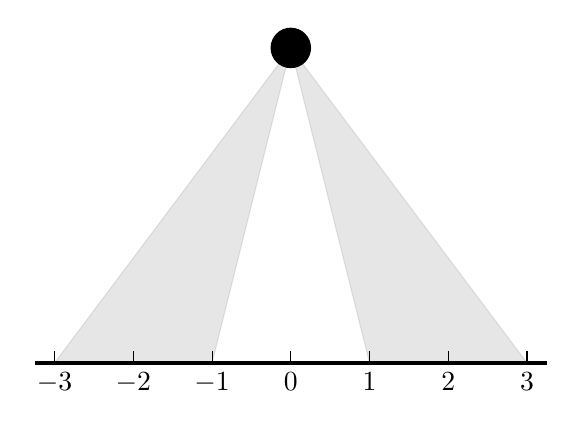
\begin{tikzpicture}
    \filldraw[opacity=0.2, color=gray] (0,4) -- (3,0) -- (1,0) -- cycle;
    \filldraw[opacity=0.2, color=gray] (0,4) -- (-3,0) -- (-1,0) -- cycle;
    \filldraw (0,4) circle (0.25);
    \draw[very thick] (-3.25,0) -- (3.25,0);
    \foreach \x in {-3,...,3}
    {
        \draw (\x,0.15) -- (\x,0);
        \node at (\x,0) [below] {$\x$};
    }

\end{tikzpicture}
\caption{ဘောလုံးကျလာနိုင်တဲ့နေရာ} 
\label{fig:balldir}
\end{figure}

\subsection*{\fSubSecCodeBf{Breakout} Class}
\fCode{Breakout} ကလပ်စ်ကို ဆက်ကြည့်ရအောင်။ ဂိမ်းရဲ့ အဓိက \fCode{View} ဖြစ်ပြီး အရှုံးအနိုင်ဆုံးဖြတ်တာ၊ ဘောလုံးနဲ့ အုတ်ခဲ၊ ဘောလုံးနဲ့ \fEn{paddle} တိုက်မိတာ စတာတွေကို ဒီကလပ်စ်မှာ ရေးထားတာပါ။ \fEn{paddle} ကို မောက်စ်နဲ့  ရွှေ့လို့ရအောင် \fCode{on\_mouse\_motion} ကလည်း ဒီထဲမှာပဲ။ $\big\llbracket$\fCode{Breakout} ကလပ်စ် အပြည့်အစုံကို စာမျက်နှာ (\fRefNo{\pageref{lst:breakout}}) မှာ ကြည့်ပါ$\big\rrbracket$။ 

\mintinline{text}|__init__| မက်သဒ်က သိပ်ရှုပ်ရှုပ်ထွေးထွေး မရှိဘူး။ မောက်စ်ပွိုင်တာ ပေါ်နေအောင်  \fCode{self.win\allowbreak dow.set\_mouse\_visible(True)} နဲ့ လုပ်ထားတယ်။ ဖျောက်ထားချင်ရင် \fCode{False} ထည့်ပေး။ \fEn{Instance variable} တွေ အားလုံးကို \fCode{None} ထည့်ထားတယ်။
%
\begin{py}
def __init__(self):
    super().__init__()

    arcade.set_background_color(WHITE)
    self.window.set_mouse_visible(True)
    self._ball = None
    self._paddle = None
    self._brick_lst = None
    self._brick_remains = None
    self._next_view = None
\end{py}
%

\fEn{Initialization} ကို \fCode{setup} မက်သဒ်မှာ အဓိက လုပ်ထားတယ်။ \mintinline{text}|__init__| မှာ ဘာလို့ မလုပ်လဲ မေးစရာရှိတယ်။ \mintinline{text}|__init__| မက်သဒ်က အော့ဘ်ဂျက် ဖန်တီးတဲ့အခါမှာပဲ အလိုအလျောက်ခေါ်ပေးတာ။ တိုက်ရိုက်ခေါ်ရတဲ့ မက်သဒ်မဟုတ်ဘူး။ ရှုံးသွားလို့ (သို့) နိုင်သွားလို့ နောက်တစ်ခါ ပြန်ဆော့ချင်ရင် အစအနေအထား ဖြစ်အောင် \fCode{setup} မက်သဒ်ကို ခေါ်လို့ရမယ်။ (ဒီတော့ \fCode{Breakout} အော့ဘ်ဂျက် အသစ်တစ်ခု ဖန်တီးတာ၊ \mintinline{text}|__init__| ကို တိုက်ရိုက်လည်း မခေါ်ဘဲ ပြန်စချင်ရင် \fCode{setup} ကို ခေါ်လို့ရမယ်)။ ရှေ့မှာတွေ့ခဲ့တဲ့ \fCode{setup\_ball}\fEn{,} \fCode{setup\_paddle}\fEn{,} \fCode{setup\_bricks} တို့ကို တစ်ဆင့် ပြန်ခေါ်ထားတာ တွေ့ရမယ်။ \fCode{\_brick\_remains} က လက်ကျန်အုတ်ခဲ အရေအတွက် မှတ်ထားဖို့။ အုတ်ခဲ တစ်လုံးပျက်သွားတိုင်း တစ်လျှော့ပေးရမယ်။

%
\begin{py}
def setup(self):
    self._paddle = arcade.SpriteSolidColor(PDL_WIDTH,
                                            PDL_HEIGHT,
                                            BLACK)
    self._paddle.bottom = PDL_Y_OFFSET
    self._paddle.center_x = CENTER_X

    self._ball = setup_ball()
    self._brick_lst = setup_bricks()
    self._brick_remains = 20
\end{py}
%

\fCode{draw} မက်သဒ်က ဂိမ်းမှာပါတဲ့ အုတ်နံရံ၊ ဘောလုံးနဲ့ \fEn{paddle} ပြားတို့ကို ဆွဲတယ်။ ဒီမက်သဒ်က \fCode{Breakout} ကလပ်စ်မှာ ထပ်ဖြည့်ထားတာ။ \fCode{View} ကလပ်စ်ရဲ့ တစ်စက္ကန့် အကြိမ်ခြောက်ဆယ် ခေါ်နေမဲ့  \fCode{on\_draw} ကို \fEn{override} လုပ်တာ မဟုတ်ဘူး။ \fCode{draw} ကို ခွဲထုတ်ထားရတာက လိုတဲ့အချိန်မှာ ကိုယ်တိုင်ခေါ်လို့ရအောင် ရည်ရွယ်တာပါ။ 
%
\begin{py}
def on_draw(self):
    self.draw()

def draw(self):
    self.clear()
    self._paddle.draw()
    self._brick_lst.draw()
    self._ball.draw()
\end{py}
%

ဂိမ်းရဲ့ အဓိကလော့ဂျစ်ကို \fCode{on\_update} မက်သဒ်မှာ တွေ့ရမှာပါ။ \fCode{View} ကလပ်စ်ရဲ့ \fCode{on\_update} ကို \fEn{override} လုပ်ပေးတာပါ။
%
\begin{py}
def on_update(self, delta_time):
    self._ball.update()
    self._paddle.update()
    self._brick_lst.update()
    bricks_hit = arcade.check_for_collision_with_list(self._ball,
                                                        self._brick_lst)
    if len(bricks_hit) > 0:
        self._ball.change_y *= -1
    for brick in bricks_hit:
        brick.remove_from_sprite_lists()
        self._brick_remains -= 1

    if self._brick_remains == 0:
        self._next_view._msg = "You Win!"
        self.window.show_view(self._next_view)

    if self._ball.center_y <= PDL_Y_OFFSET:
        self._next_view._msg = "You Lost!"
        self.window.show_view(self._next_view)

    if (arcade.check_for_collision(self._ball, self._paddle)
            and self._ball.change_y < 0):
        self._ball.change_y *= -1
\end{py}
%
\fCode{on\_update} ကို တစ်စက္ကန့် အကြိမ်ခြောက်ဆယ် အဆက်မပြတ် အလိုအလျောက် ခေါ်ပေးတယ်လို့ ပြောခဲ့တာ ပြန်အမှတ်ရမယ် ထင်ပါတယ်။ ဂိမ်းရဲ့ \fEn{state} ကို ဒီမက်သဒ် တစ်ကြိမ်ခေါ်တိုင်း \fEn{update} လုပ်ပေးရပါမယ်။ ဒါဟာ ဂိမ်းတစ်ခုရဲ့ အချိန်နဲ့အမျှ ပြောင်းလဲနေတဲ့ အရာအားလုံးအတွက် အဓိကသော့ချက်ပဲ။   ပထမဆုံး \fEn{Breakout} မှာပါတဲ့ ဘောလုံး၊ \fEn{paddle} နဲ့ အုတ်ခဲအားလုံးရဲ့ လက်ရှိအခြေအနေကို \fEn{update} လုပ်ရမယ်။ ဒီအတွက် ဂိမ်းမှာပါဝင်တဲ့ သက်ဆိုင်ရာ \fCode{Sprite} (သို့) \fCode{SpriteList} အားလုံးရဲ့ \fCode{update} မက်သဒ်ကို ခေါ်ပေးရမှာပါ။
%
\begin{py}
self._ball.update()
self._paddle.update()
self._brick_lst.update()
\end{py}
%

\fCode{check\_for\_collision\_with\_list} က ဝင်တိုက်မိတဲ့ \fCode{Sprite} တွေကို စစ်ထုတ်ပေးတဲ့ မက်သဒ်။ ဘောလုံးနဲ့ တိုက်မိတဲ့ အုတ်ခဲတွေကို လိုချင်တာ။ ဒီတော့ အခုလို ခေါ်ရမယ် 
%
\begin{py}
bricks_hit = arcade.check_for_collision_with_list(self._ball,
                                                  self._brick_lst)
\end{py}
%

အုတ်ခဲ (တွေ) နဲ့ ဝင်တိုက်ရင် ဘောလုံးကို အထက် (သို့) အောက် ပြန်ကန်ထွက်အောင် \fCode{change\_y} ကို လက္ခဏာ ဆန့်ကျင်ဘက် ပြောင်းပေးပါတယ်။
%
\begin{py}
if len(bricks_hit) > 0:
    self._ball.change_y *= -1
\end{py}
%
ဝင်တိုက်တဲ့ အုတ်ခဲတွေကို ဖျက်ပစ်ရပါမယ်။ ဖျက်လိုက်ရင် လက်ကျန်အုတ်ခဲလည်း လျော့သွားရမယ်။ ဒီအတွက် အခုလို
%
\begin{py}
for brick in bricks_hit:
    brick.remove_from_sprite_lists()
    self._brick_remains -= 1
\end{py}
%
တိုက်မိတဲ့ အုတ်ခဲတစ်ခဲချင်း ဖယ်ထုတ်ပါတယ်။

\subsection*{Start, Main and End \fSubSecCodeBf{View}s}
ပထမ စစချင်းမှာ ပုံ (\fRefNo{\ref{fig:breakout}}) မှာ တွေ့ရတဲ့ အနေအထားအတိုင်း ရှိနေမယ်။ ဒါပေမဲ့ စတာနဲ့ ဘောလုံးက ချက်ချင်းထွက်ရင် ဆော့ရတာ သိပ်အဆင်မပြေဘူး။ ကလစ်နှိပ်လိုက်မှ ဘောလုံးစထွက်မယ်ဆိုရင် ပိုကောင်းမယ်။ \fCode{StartView} ကို အခုလိုသတ်မှတ်ထားတယ်
%
\begin{py}
class StartView(arcade.View):
    def __init__(self):
        super().__init__()
        self._next_view = None

    def on_draw(self):
        self.clear()
        # ß Breakout \fMM{ရဲ့} setup \fMM{နဲ့} draw \fMM{ကိုခေါ်တာ}ß
        self._next_view.setup()
        self._next_view.draw()

    def on_mouse_press(self, x, y, button, modifiers):
        # ß\fMM{ကလစ်နှိပ်ရင်} Breakout View \fMM{ကို ပြောင်းပေးတာ}ß
        if self._next_view:
            self._next_view.setup()
            self.window.show_view(self._next_view)
\end{py}
%
စောစောကရှင်းပြခဲ့တဲ့ \fCode{Breakout} ဟာ ဂိမ်းရဲ့ အဓိက \fCode{View} ။ ဒါပေမဲ့ ဒီ \fCode{View} က စတာနဲ့ ဘောလုံးက ရွေ့မှာ \fCode{on\_draw} နဲ့  \fCode{on\_update} က ရပ်ထားလို့မရဘူး။ \fCode{View} ကို \fCode{Window} မှာ ပြပြီဆိုတာနဲ့ တောက်လျှောက် ခေါ်နေမှာ။ \fCode{StartView} က ရုပ်ပုံကို အငြိမ်ပဲ ပြပေးရမယ်။ ဖြစ်နိုင်တဲ့ နည်းလမ်းတစ်ခုက \fCode{Breakout} ရဲ့ \fCode{setup} နဲ့ \fCode{draw} ကို \fCode{StartView} ရဲ့ \fCode{on\_draw} ကနေ ခေါ်လို့ရပါတယ်။ \fCode{StartView} နဲ့ \fCode{Breakout} ကို \fCode{main} မက်သဒ်ထဲမှာ အခုလို ချိတ်ပေးထားပါမယ်။ 
%
\begin{py}
start_view = StartView()
game_view = Breakout()
# ...
start_view._next_view = game_view
window.show_view(start_view)
# ...
\end{py}
%

အရှုံးအနိုင် \fEn{You Win!/You Lose!} ပြဖို့ \fCode{EndView} ရဲ့ တာဝန်။ ရှုံး (သို့) နိုင်ရင် \fOpn{မက်ဆေ့ချ်} ပြပေးပြီး တစ်ခါထပ်ဆော့ချင်ရင် ကလစ်နှိပ်ရပါမယ်။  
%
\begin{py}
class EndView(arcade.View):
    def __init__(self):
        super().__init__()
        self._next_view = None
        self._msg = None

    def on_draw(self):
        self.clear()
        arcade.draw_text(self._msg,
                         WIN_WIDTH / 2,
                         WIN_HEIGHT / 2,
                         RED,
                         font_size=20,
                         anchor_x="center")

    def on_mouse_press(self, x, y, button, modifiers):
        if self._next_view:
            self.window.show_view(self._next_view)
\end{py}
%
\fCode{main} မက်သဒ်ထဲမှာ အခုလို ချိတ်ပေးထားပါတယ်
%
\begin{py}
end_view = EndView()
# ...
end_view._next_view = start_view
\end{py}
%


\subsection*{နိဂုံး}
ဒီအခန်းမှာ \fEn{Breakout} ဂိမ်းကို အသုံးချ ဥပမာအနေနဲ့ ထည့်ပေးထားတဲ့ ရည်ရွယ်ချက်က \fEn{Arcade} လိုက်ဘရီနဲ့ ဂိမ်းတွေ ဖန်တီးနိုင်ဖို့ အဓိက မဟုတ်ပါဘူး။ \fEn{Inheritance} ကို လိုက်ဘရီတွေမှာ အသုံးချလေ့ရှိတဲ့ ပုံစံတချို့ကို နားလည်သဘောပေါက်အောင်၊ သတိပြုမိအောင်၊ ဆက်စပ်မိအောင် အဓိက ရည်ရွယ်တာပါ။ စလေ့လာသူတွေအတွက် လွယ်လွယ်နဲ့ နားလည်နိုင်မယ်လို့တော့ မမျှော်လင့်နိုင်ဘူး။ စိတ်ရှည်ရှည်ထား အချိန်ပေးပြီး နားလည်သဘောပေါက်အောင် လေ့လာဖို့ လိုပါလိမ့်မယ်။ ပရိုဂရမ်အပြည့်အစုံကို အောက်မှာ ဖော်ပြပေးထားပါတယ်။ 

တည်နေရာ အတွက်အချက်တွေ နားမလည်လို့လည်း သင်္ချာကြောက်သူတွေ စိတ်ဓါတ်ကျစရာ မလိုပါဘူး။ အတွက်အချက်တွေ အကြမ်းဖျဉ်းလောက် နားလည်အောင် ကြည့်၊ ကျန်တဲ့ ပရိုဂရမ်းမင်းနဲ့ဆိုင်တဲ့ သဘောတရားတွေ အဓိကထား ကြည့်မယ်ဆိုရင်လည်း အတိုင်းအတာတစ်ခုထိ အကျိုးရှိမှာပါပဲ။

%
\begin{py}
ß\label{lst:breakoutfull}ß
import random
import arcade
from arcade.color import *

WIN_WIDTH = 400
WIN_HEIGHT = 600

PDL_WIDTH = 60
PDL_HEIGHT = 10
PDL_Y_OFFSET = 30    # distance between paddle and lower edge of window

BALL_RADIUS = 10
BRICKS_PER_ROW = 10
BRICK_ROWS = 10      # number of brick rows
BRICK_GAP = 4        # gap between bricks
BRICK_WIDTH = ((WIN_WIDTH - (BRICKS_PER_ROW - 1) * BRICK_GAP)
               // BRICKS_PER_ROW)
LEFT_MARGIN = (WIN_WIDTH - (BRICK_WIDTH * BRICKS_PER_ROW +
                            BRICK_GAP * (BRICKS_PER_ROW - 1))) // 2
BRICK_HEIGHT = 8
BRICK_Y_OFFSET = 414
CENTER_X = WIN_WIDTH // 2
CENTEr_Y = WIN_HEIGHT // 2

ß\label{lst:breakout}ß
class Breakout(arcade.View):
    def __init__(self):
        super().__init__()

        arcade.set_background_color(WHITE)
        self.window.set_mouse_visible(True)
        self._ball = None
        self._paddle = None
        self._brick_lst = None
        self._brick_remains = None
        self._next_view = None

    def setup(self):
        self._paddle = arcade.SpriteSolidColor(PDL_WIDTH,
                                               PDL_HEIGHT,
                                               BLACK)
        self._paddle.bottom = PDL_Y_OFFSET
        self._paddle.center_x = CENTER_X

        self._ball = setup_ball()
        self._brick_lst = setup_bricks()
        self._brick_remains = 20

    def on_draw(self):
        self.draw()

    def draw(self):
        self.clear()
        self._paddle.draw()
        self._brick_lst.draw()
        self._ball.draw()

    def on_update(self, delta_time):
        self._ball.update()
        self._paddle.update()
        self._brick_lst.update()
        bricks_hit = arcade.check_for_collision_with_list(self._ball,
                                                          self._brick_lst)
        if len(bricks_hit) > 0:
            self._ball.change_y *= -1
        for brick in bricks_hit:
            brick.remove_from_sprite_lists()
            self._brick_remains -= 1

        if self._brick_remains == 0:
            self._next_view._msg = "You Win!"
            self.window.show_view(self._next_view)

        if self._ball.center_y <= PDL_Y_OFFSET:
            self._next_view._msg = "You Lost!"
            self.window.show_view(self._next_view)

        if (arcade.check_for_collision(self._ball, self._paddle)
                and self._ball.change_y < 0):
            self._ball.change_y *= -1

    def on_mouse_motion(self, x, y, dx, dy):
        self._paddle.center_x = x


def setup_bricks():
    colors = [CYAN, CYAN, GREEN, GREEN, GOLD, GOLD,
              ORANGE, ORANGE, RED, RED]
    brick_lst = arcade.SpriteList()
    x = LEFT_MARGIN + BRICK_WIDTH // 2
    y = BRICK_Y_OFFSET + BRICK_HEIGHT // 2
    # 10 x 10 bricks wall
    for i in range(BRICKS_PER_ROW):
        for j in range(BRICK_ROWS):
            brick = arcade.SpriteSolidColor(BRICK_WIDTH,
                                            BRICK_HEIGHT,
                                            colors[i])
            brick.center_x = x + (j * (BRICK_WIDTH + BRICK_GAP))
            brick.center_y = y + (i * (BRICK_HEIGHT + BRICK_GAP))
            brick_lst.append(brick)
    return brick_lst


class Ball(arcade.SpriteCircle):
    def update(self):
        self.center_y += self.change_y
        self.center_x += self.change_x

        if self.left < 0:
            self.change_x *= -1

        if self.right > WIN_WIDTH:
            self.change_x *= -1

        # hitting bottom edge doesn't bounce
        if self.bottom < 0:
            pass

        if self.top > WIN_HEIGHT:
            self.change_y *= -1


def setup_ball():
    ball = Ball(BALL_RADIUS, arcade.color.BLACK)
    ball.center_x = WIN_WIDTH // 2
    ball.center_y = WIN_HEIGHT // 2
    ball.change_y = -6
    random.uniform(1.0, 3.0)
    ball.change_x = random.uniform(1.0, 3.0) \
        if random.uniform(0.0, 1.0) <= 0.5 \
        else random.uniform(-1.0, -3.0)
    return ball


class StartView(arcade.View):
    def __init__(self):
        super().__init__()
        self._next_view = None

    def on_draw(self):
        self.clear()
        self._next_view.setup()
        self._next_view.draw()

    def on_mouse_press(self, x, y, button, modifiers):
        if self._next_view:
            self._next_view.setup()
            self.window.show_view(self._next_view)


class EndView(arcade.View):
    def __init__(self):
        super().__init__()
        self._next_view = None
        self._msg = None

    def on_draw(self):
        self.clear()
        arcade.draw_text(self._msg,
                         WIN_WIDTH / 2,
                         WIN_HEIGHT / 2,
                         RED,
                         font_size=20,
                         anchor_x="center")

    def on_mouse_press(self, x, y, button, modifiers):
        if self._next_view:
            self.window.show_view(self._next_view)


def main():
    window = arcade.Window(WIN_WIDTH, WIN_HEIGHT, "Breakout")
    start_view = StartView()
    game_view = Breakout()
    end_view = EndView()

    start_view._next_view = game_view
    game_view._next_view = end_view
    end_view._next_view = start_view

    window.show_view(start_view)
    arcade.run()


if __name__ == "__main__":
    main()

\end{py}
%
